\subsection{Collections}
\textit{Compare/contrast use of ArrayList / LinkedList / HashMap / HashSet / TreeSet}

Collections are Objects that can hold other objects. They are useful for temporarily storing a group of objects in memory, and processing them somehow. Collections hold several objects of the same class. 

Collections provide functionality such as adding objects, removing objects, sorting, iterating, and counting the amount of objects.

In the graph below we can see the inheritance hierarchy of some Java collections; ArrayList, LinkedList, HashMap, HashSet, and TreeSet. There are three basic types, namely sets, lists, and maps.

\subsubsection{Sets}
Sets usually don't allow duplicate elements, As in a mathematical set, there is no implicit order of elements. Subclasses, such as the TreeSet may implement ordering.\cite{set}

\subsubsection{Lists}
A lists in java is an ordered collection. The elements in the list have an index that can be used to insert (into a specific position) or access the element. Lists allow duplicate elements. The index is 0-based. Sometimes null elements are allowed.\cite{list}

\subsubsection{Maps}
A map is an object that maps keys to values, in one-to-one fashion. Maps cannot contain duplicate keys. \cite{map}

There is no guarantee in the order of elements in a map. In fact the order might change as elements are added or removed.  \cite{map}

\begin{figure}[H]\centering
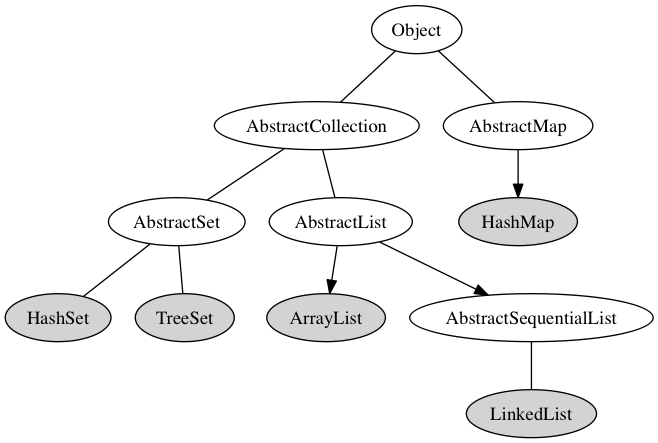
\includegraphics[width=\linewidth]{collections.png}
\caption{Some Java Collections}
\label{fig:collections}
\end{figure}
A summary of some of Java collections:
\begin{table}[!htb]
\centering
\begin{tabulary}{\columnwidth}{ |>{\raggedright\arraybackslash} p{0.2\columnwidth} | >{\raggedright\arraybackslash}p{0.1\columnwidth} | >{\raggedright\arraybackslash}p{0.1\columnwidth} | >{\raggedright\arraybackslash}p{0.4\columnwidth}|}
\hline
\textbf{Collection} & \textbf{Nulls} & \textbf{Access Cost}& \textbf{Notes} \\ \hline 
TreeSet  & Yes  & log(n) & Not Synchronized. Natural ordering. \\ \hline 
ArrayList  & Yes &   O(1) & Not Synchronized. Insert ordering.\\ \hline 
LinkedList  & Yes &  O(n) & Not Synchronized. Insert ordering.\\ \hline 
HashMap  & Yes & O(1) & Null value or null key. Not Synchronized. \\ \hline 
HashSet  & Yes & O(1) & Not Synchronized.  \\ \hline 
\end{tabulary}
\caption{Comparison of Some Java Collections}\label{tab:collections}
\end{table}

I compared ArrayList, LinkedList, HashMap, HashSet, and TreeSet by adding 100,000 elements to them, removing 10,000 non-subsequent elements, finding 10,000 non-subsequent elements, and clearing the entire collection. See page \pageref{App:AppendixE} for the sample program.

The performance differences clearly divide the collections in to groups matching their based class.

\subsubsection{Adding Elements}
Although the HashSet and TreeSet took more time to add 10,000 elements, (twice and three times, respectively) they still were quite fast. HashSet took 13ms and TreeSet took 20ms.

\subsubsection{Removing Elements}
ArrayList and LinkedList were the slowest collections when it comes to removing an element. ArrayList was almost 250 times slower (498ms) and LinkedList was 600 times slower (1272ms) than a HashMap.

A LinkedList is really a doubly-linked list, so iteration can start from either the beginning or the end of the list. But still, it needs to iterate through maximum half of the elements to find the element to remove.
%To be fair, I removed the element by value, not by index. So, index 4 might have a value "Hello". I removed the object "Hello", without knowing its index. Removing by index is certainly faster than by value of the object, for lists.

\subsubsection{Finding and Element}
Logically, finding an element by value was similar to deleting. The lists were significantly slower.

\subsubsection{Clearing the Collection}
All collections performed similarly when clearing all elements. All were fast, although just like adding, the sets were slower.

%columns
% 1- ArrayList
% 2 - Linkedlist
% 3 - HashMap
% 4 - HashSet
% 5 - TreeSet

%rows
% 0 - Add
% 1 - Remove
% 2 - Find
% 3 - clear
\makeatletter
\pgfplotsset{
    calculate offset/.code={
        \pgfkeys{/pgf/fpu=true,/pgf/fpu/output format=fixed}
        \pgfmathsetmacro\testmacro{(\pgfplotspointmeta *10^\pgfplots@data@scale@trafo@EXPONENT@y)*\pgfplots@y@veclength)}
        \pgfkeys{/pgf/fpu=false}
    },
    every node near coord/.style={
        /pgfplots/calculate offset,
        yshift=-\testmacro                      
    },
    every node near coord/.append style={font=\tiny},
}
\pgfplotstableread{
0 6   4    3   13   20
1 498 1272 2   2    7
2 914 2431 1   1    4
3 1   2    0   1    0


%1 6  498  914  1
%2 4  1272 2431 2
%3 3  2    1    0
%4 13 2    1    1
%5 20 7    4    0

}\dataset
\begin{tikzpicture}
\begin{axis}[ybar,
bar width=4.5,
width=0.9\columnwidth,
        ymin=0,
        ymax=2500,        
        ylabel={ms},
        xtick=data,
        xticklabels = {
            Add,
            Remove,
            Find,
            Clear
        },
        xticklabel style={yshift=-5ex},
        major x tick style = {opacity=0},
        minor x tick num = 1,
        minor tick length=1ex,
        every node near coord/.append style={
                anchor=east,
                rotate=90
        }      
        ]
\addplot[draw=black,fill=black!20, nodes near coords=ArrayList] table[x index=0,y index=1] \dataset; %Data1
\addplot[draw=black,fill=black!40, nodes near coords=LinkedList] table[x index=0,y index=2] \dataset; %Data2
\addplot[draw=black,fill=black!60, nodes near coords=HashMap] table[x index=0,y index=3] \dataset; %Data3
\addplot[draw=black,fill=black!80, nodes near coords=HashSet] table[x index=0,y index=4] \dataset; %Data3
\addplot[draw=black,fill=black!100, nodes near coords=TreeSet] table[x index=0,y index=5] \dataset; %Data3
\end{axis}
 \end{tikzpicture}
 
Overall, the HashMap was the fastest collection. It uses a key to access each element directly, without iterating.